\section{Introduction}
The binary information in a digital computer must have a physical existence in some medium for storing individual bits. A binary cell is a device that possesses two stable states and is capable of storing one bit (0 or 1) of information. Bit is a binary digit with only 2 discrete values 0 \& 1. Digital system is an interconnection of digital modules. These manipulate discrete quantities of information that are represented in binary form.

\section{Number representation}
A number can be expressed in a specific number system. A general representation in a base-r system is:\\
\[ a_n*r^n + a_{n-1}*r^{n-1} + .... + a_1*r + a_0\]\
\[+ a_{-1}*r^{-1} + a_{-2}*r^{-2} + ....\]
where, r is a base of the number system \& \\
\(a_{i}\) = coefficients of bases with values varying from 0 to r-1 

\section{Number base conversion}
\subsection{Decimal}
If a number includes a radix point, the number is split into an integer and a fraction part. Then conversion of decimal integer to a number in base-r is done by dividing the number and all successive quotients by r and accumulating the reminders. In case of fractions, multiplication is used instead of division 

\subsection{Binary, Octal, Hexadecimal} 
\subsubsection{Binary Octal Conversion}
Binary to Octal Conversion:  Clubbing 3 bits to obtain a single Octal digit.\\
Octal to Binary Conversion:  Replace octal digit into corresponding 3 binary digits.

\subsubsection{Binary Hexadecimal Conversion}
Binary to HEX Conversion:  Clubbing 4 bits to obtain a single Hex digit.\\
HEX to Binary Conversion:  Replace Hex digit into corresponding 4 binary digits.
\clearpage

\section{Complements of numbers}
Complements are used in digital systems to simplify the subtraction operation and logical manipulation. There are 2 types of complements:
\begin{enumerate}
    \item \textbf{Radix complement (r's complement):} r's complement of an n digit number N in base-r is defined as \(r^n-n\) for N != 0 and 0 for N = 0. \\  r's complement = (r-1)'s complement + 1
    \item \textbf{Diminished radix complement ((r-1)'s complement):} (r-1)'s complement of an n-digit number N in base-r is defined as \( (r^{n} -1 ) - N \) where, r is base number.
    \begin{itemize}
        \item 1's complement = toggling bits 
        \item 0's complement = subtracting every digit from 9
    \end{itemize}
\end{enumerate}
Complement of the complement restores the number to its original value.

\subsection{subtraction using complements}
M \& N are n-digit unsigned numbers in base-r.\\
M - N = M + (r's complement of N)

\textbf{if M \( \geqslant \) N} : M - N = M + (r's complement of N) + \(r^{n}\); Carry can be ignored.\\
\textbf{if M < N} : M - N = \(r^{n}\) - (N- M)\\ 
= r's complement of (N-M) (answer) result is negative.\\
= - (r's complement of answer) (familiar representation)

\section{Signed Binary Numbers} 
\subsection{Ordinary Arithmatic}
In ordinary arithmatic, negative numbers are represented with a minus sign. But due to hardware limitations, Computers must represent everything with binary digits.\\ 
Signed Binary Numbers representation with sign bit = 0 for a positive number; sign bit = 1 for a negative number\\
\begin{table}[H]
\centering
\begin{tabular}{ll}
\hline
\multicolumn{1}{|l|}{\textbf{sign bit}} & \multicolumn{1}{l|}{\textbf{Number (magnitude)}} \\ \hline
\end{tabular}
\end{table}

Unsigned number: Leftmost bit is the MSB\\
Signed number: Left most bit is the sign bit.
Eg. 01001 = 9 (unsigned) \& + 9 (signed)\\
11001 = 25 (unsigned) \&  -9 (signed)

\par This representation is known as the signed magnitude convention, or ordinary arithmatic. 

\subsection{Signed Complement System}
In this representation, a negative number is indicated by its compliment Negative number in Signed Complement System representation:\\
\begin{table}[H]
\centering
\begin{tabular}{ll}
\hline
\multicolumn{1}{|l|}{\textbf{sign bit}} & \multicolumn{1}{l|}{\textbf{Complement}} \\ \hline
\end{tabular}
\end{table}

Positive number in Signed Complement System representation:\\
\begin{table}[H]
\centering
\begin{tabular}{ll}
\hline
\multicolumn{1}{|l|}{\textbf{sign bit}} & \multicolumn{1}{l|}{\textbf{Number}} \\ \hline
\end{tabular}
\end{table}
Complement could be (l's or 2's) but usually 2's complement.\\
eg. Three different representations for -9
\begin{itemize}
    \item Signed magnitude: 1-0001001 (Changing the leftmost bit)
    \item Signed is compliment: 1-1110110 (Complement of all the bits including sign bit)
    \item Signed as compliment: 1-1110111 (Complement of all the bits \& add 1)
\end{itemize}
(Add table 1.3 to Notes) 

\subsection{Addition of signed numbers}
\begin{itemize}
    \item Signed Magnitude: 
    \begin{itemize}
        \item if signs are same: 
        \begin{itemize}
            \item Subtract magnitude.
            \item Keep the sign.
        \end{itemize}
        \item if signs are different: 
        \begin{itemize}
            \item Compare the numbers.
            \item Subtract smaller one from the larger one.
            \item Append sign of the larger number.
        \end{itemize}
    \end{itemize}
    \item Signed 2's complement: simply add the numbers including sign bit and discard the carry. 
\end{itemize}
 
\subsection{Subtraction of signed numbers}
2's complement of subtrahend (including sign bit) is added to the minuend (including sign bit) and discard the carry. 

As subtraction \& addition basically use the same method in a signed 2's complement representation. Computers need only one common hardware to handle both types of arithmatic.

\clearpage
\section{Binary codes}
\subsection{Binary coded Decimal code (BCD)}
Decimal number representation in binary (4 bits are used to represent a decimal digit). Binary combination 0000 to 1001 represent 0-9 whereas, 1010 to 1111 are not used and have no meaning in BCD.\\
\subsubsection{BCD addition}
1) Sum \( \leqslant \) 1001 (without carry)\\
\quad Sum = A + B
2) Sum \( \geqslant \) 1010\\ 
Sum = add 6 (16-10) to the binary sum and also generates a carry\\ Representation of signed BCD is similar to the signed numbers in binary.

\subsection{Gray code}
Advantage over straight binary numbers only one bit change in the next an increment. This is useful in continuous data such as ADCs 
\begin{table}[H]
\centering
\begin{tabular}{ll}
\hline
\multicolumn{1}{|l|}{\textbf{Binary Number}} & \multicolumn{1}{l|}{\textbf{Gray Code}} \\ \hline
\multicolumn{1}{|l|}{0} & \multicolumn{1}{l|}{00} \\ \hline
\multicolumn{1}{|l|}{1} & \multicolumn{1}{l|}{01} \\ \hline
\multicolumn{1}{|l|}{2} & \multicolumn{1}{l|}{11} \\ \hline
\multicolumn{1}{|l|}{3} & \multicolumn{1}{l|}{10} \\ \hline
\end{tabular}
\end{table}

\subsection{ASCII character code} 
ASCII stands for American Standard code for Information Interchange.\\
An alphanumeric character set representation with binary digits. This set includes 10 decimal digits, 26 letters of the alphabet (uppercase \& lowercase) and multiple special characters. This is a 7 bit code with but used as a byte for storing in computers. 

\subsection{Error detecting code}
A bit is added to the code to detect errors. The pit is called as parity bit. Parity bit represents total of is in the number. The parity could be odd or even.
\begin{table}[H]
\centering
\begin{tabular}{lll}
\hline
\multicolumn{1}{|l|}{\textbf{Number}} & \multicolumn{1}{l|}{\textbf{Even Parity}} & \multicolumn{1}{l|}{\textbf{Odd Parity}} \\ \hline
\multicolumn{1}{|l|}{101} & \multicolumn{1}{l|}{0101} & \multicolumn{1}{l|}{1011}\\ \hline
\multicolumn{1}{|l|}{111} & \multicolumn{1}{l|}{1111} & \multicolumn{1}{l|}{0111}\\ \hline
\end{tabular}
\end{table}

\clearpage
\section{Binary storage and registers}
The binary information in a digital computer must a physical existence in some medium for storing bits. A binary cell is a device that possesses 2 stable states and is capable of storing one bit of information (0 or 1)

\subsection{Registers} A register is a contiguous group of binary cells. An n-bit register can store n bit information, and can have \(2^{n}\) possible states. 

\subsection{Register transfer} 
A digital system is characterized by its registers and the components that perform data processing. In digital systems, a register transfer operation is a basic operation that consists of a transfer of binary information from one set of registers into another set of registers.The transfer may be direct, from one register to another, or may pass through data‐processing circuits to perform an operation. \textbf{The device most commonly used for holding data is a register, and Binary variables are manipulated by means of digital logic circuits.} 

\begin{figure}[H]
\begin{center}
    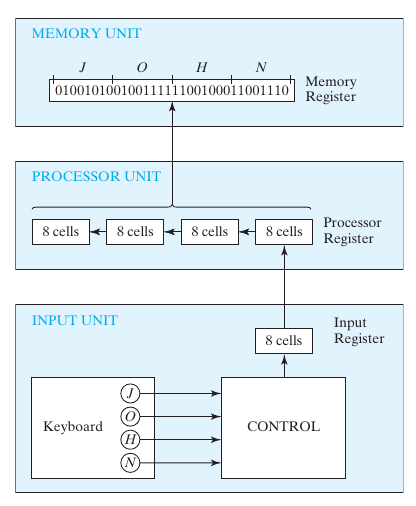
\includegraphics[width=4in]{images/RTL.png}
    \caption{Transfer of information among registers}
    \label{RTL}
\end{center}
\end{figure}

\clearpage
\section{Binary logic}
Binary logic deals with variables that take on 2 discrete values and with operations that assume logical meaning. Binary logic consists of binary variables and a set of logical operation. Each variables has only 2 distinct values 1 \& 0. Basic logical operations include only 3 functions: AND, OR \& NOT. 

\subsection{Logic gates} are the electronic circuits that operate on one or more physical input signals to produce an output signal. Binary information 
into voltage levels. Voltage ranges are assigned to logic 0 \& Logic 1 for interpretation.

\begin{figure}[H]
\begin{center}
    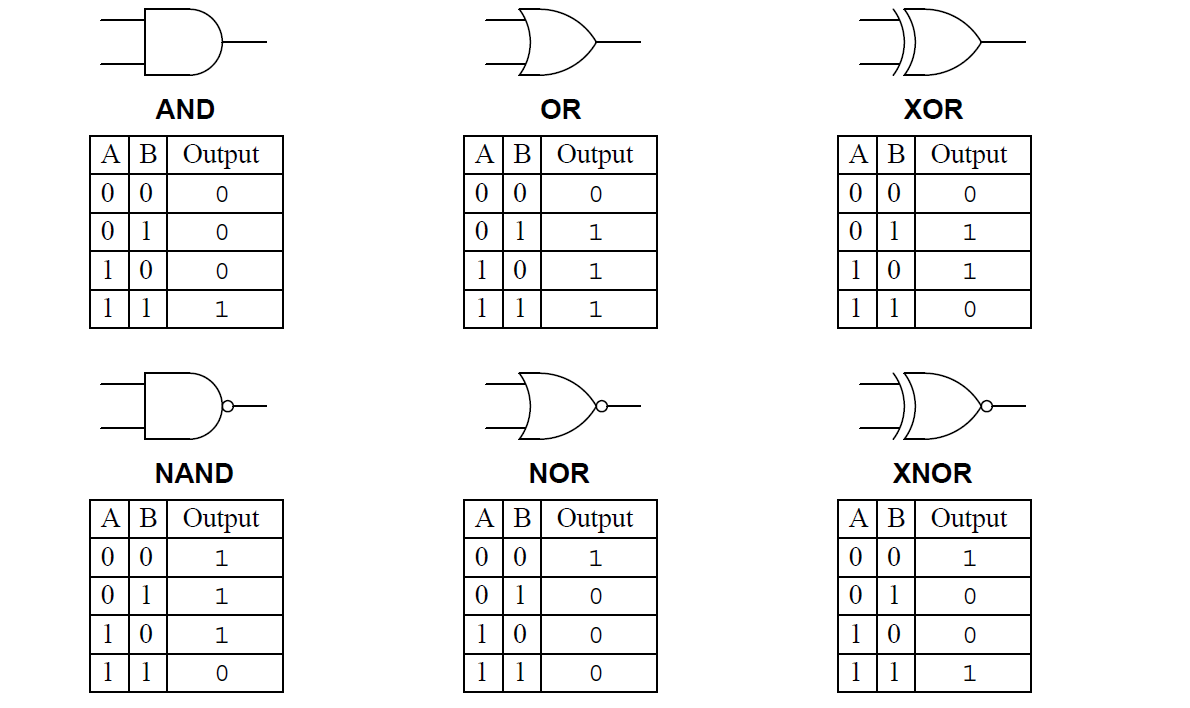
\includegraphics[width=\textwidth]{images/LogicGates.png}
    \caption{Logic Gates \& their Truth tables}
    \label{LogicGates}
\end{center}
\end{figure}